\documentclass{article}
\usepackage[utf8]{inputenc}
\usepackage{amsmath}
\usepackage{caption}
\usepackage{subcaption}
\usepackage{graphicx}
\usepackage{natbib}


\title{Weekly Report}
\author{Junior Team }
\date{July 2020}

\begin{document}

\maketitle

\section*{Introduction}

\section{Scaling Cost}
One idea that was proposed was to scale the differences of angular velocities ($\dot{\theta}_{observed}$ and $\dot{\theta}_{predicted}$) in the cost function used in \textit{fmincon}. The previous method did not account for units, and since the angular velocity changes were numerically much larger, they could dominate the optimization. In order to add a scale to our cost function, Dr. Posa suggested we use this formula:
\begin{gather}
cost = \frac{|| D *(v_{observed} - v_{predicted})||^2}{||D * v_{observed}||^2} \\[2ex]
D = 
    \left [
        \begin{array}{ccc}
             1 & 0 & 0\\
             0 & 1 & 0\\
             0 & 0 & scale\\
        \end{array} 
    \right ]
\end{gather}
\begin{figure}[h!]
\centering
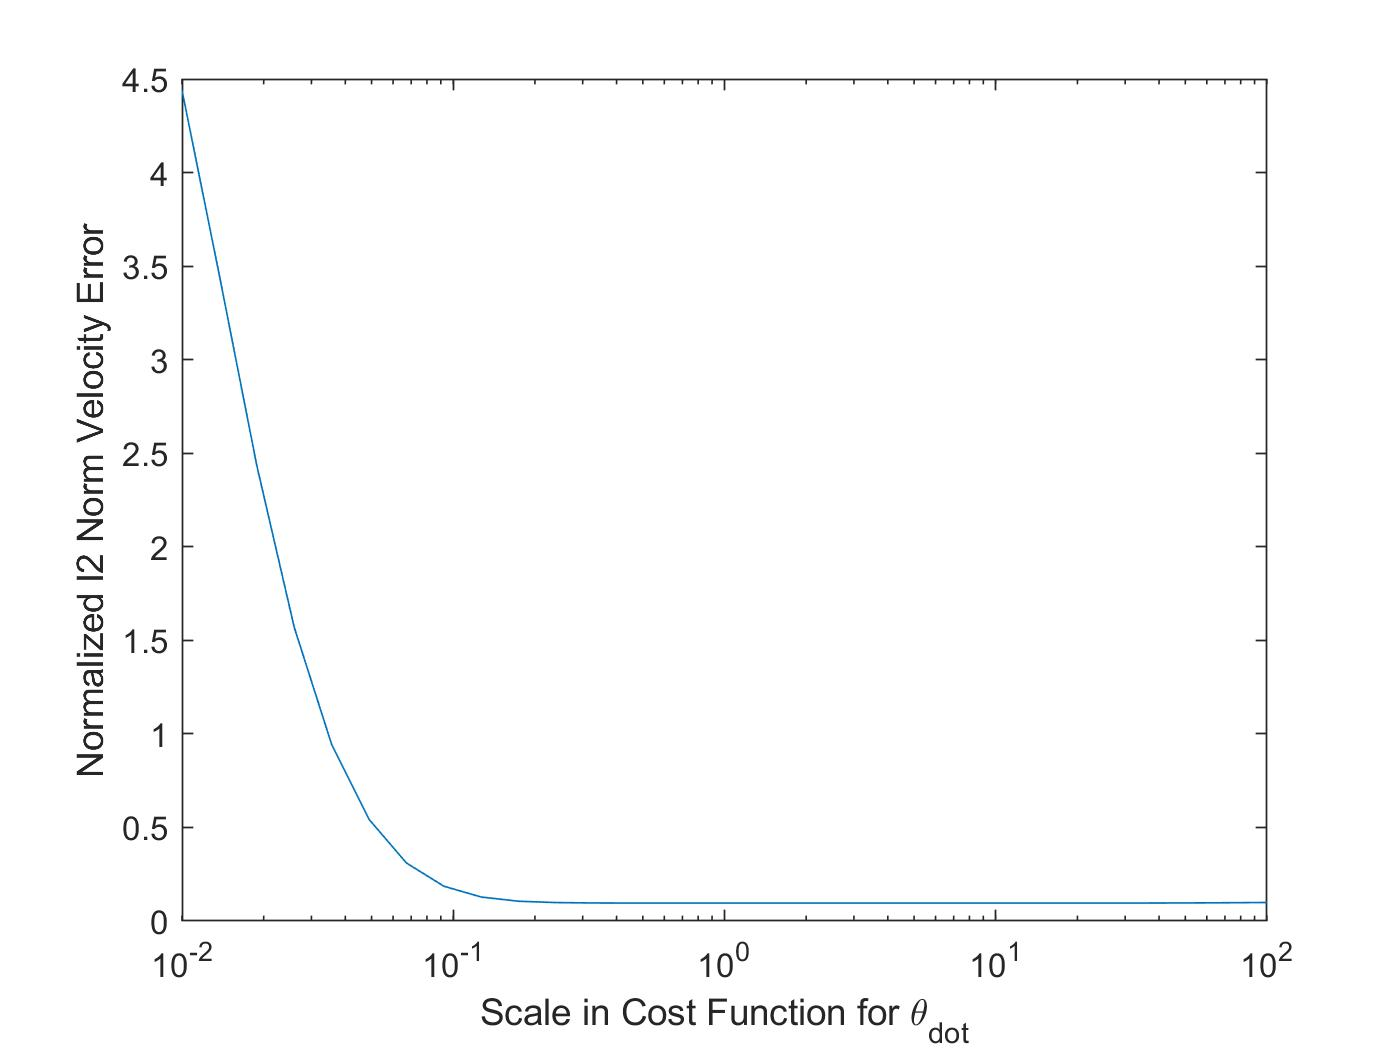
\includegraphics[scale=0.15]{scaled.jpg}
\caption{Scaling $\dot{\theta}$ Differences for IRB}
\label{fig:scaled}
\end{figure}

\noindent As the figure above shows (Fig. \ref{fig:scaled}), scaling theta dot in the updates cost function (Eq. 1) does not lower the error given by the original cost function. When Dr. Fazeli and his coauthors chose to base their error comparison on the normalized $l_2$ norm of velocity, they made an implicit choice on their definition of accuracy. Since we have been using Dr. Fazeli's data as well as referring mostly to his papers, we have also stuck to their cost function. Depending on the application of interest however, it may make sense to update the cost function to prioritize certain needs. Perhaps also, there is a better metric for judging the effectiveness of impact models. 

\section{Nonzero Error for IRB with Width }
For quite some time, Dr. Posa has been asking us why some of our IRB plots with width still have significant error, Since we have three equations and three variables we are optimizing over, we should be able to get nearly 0 cost, as long as we aren't running into any major issues with the energy constraints. It turns out some of us had different settings in \textit{fmincon} but once we all switched our step tolerance to $e^{-10}$ we were getting errors basically equal to zero (ignoring numerical and a few outliers). \\

\noindent When comparing our errors (Fig. \ref{fig:wIRB}) with the plot from \citet{nimaPaper} (Fig. \ref{fig:cIRB}), the IRB with width's error is effectively zero compared to the classical IRB which has an expected error of 0.6. 

\begin{figure}[ht]
    \caption{Comparison of Errors for IRB With and Without Width}
    \centering
    \begin{subfigure}[b]{0.45\linewidth}
        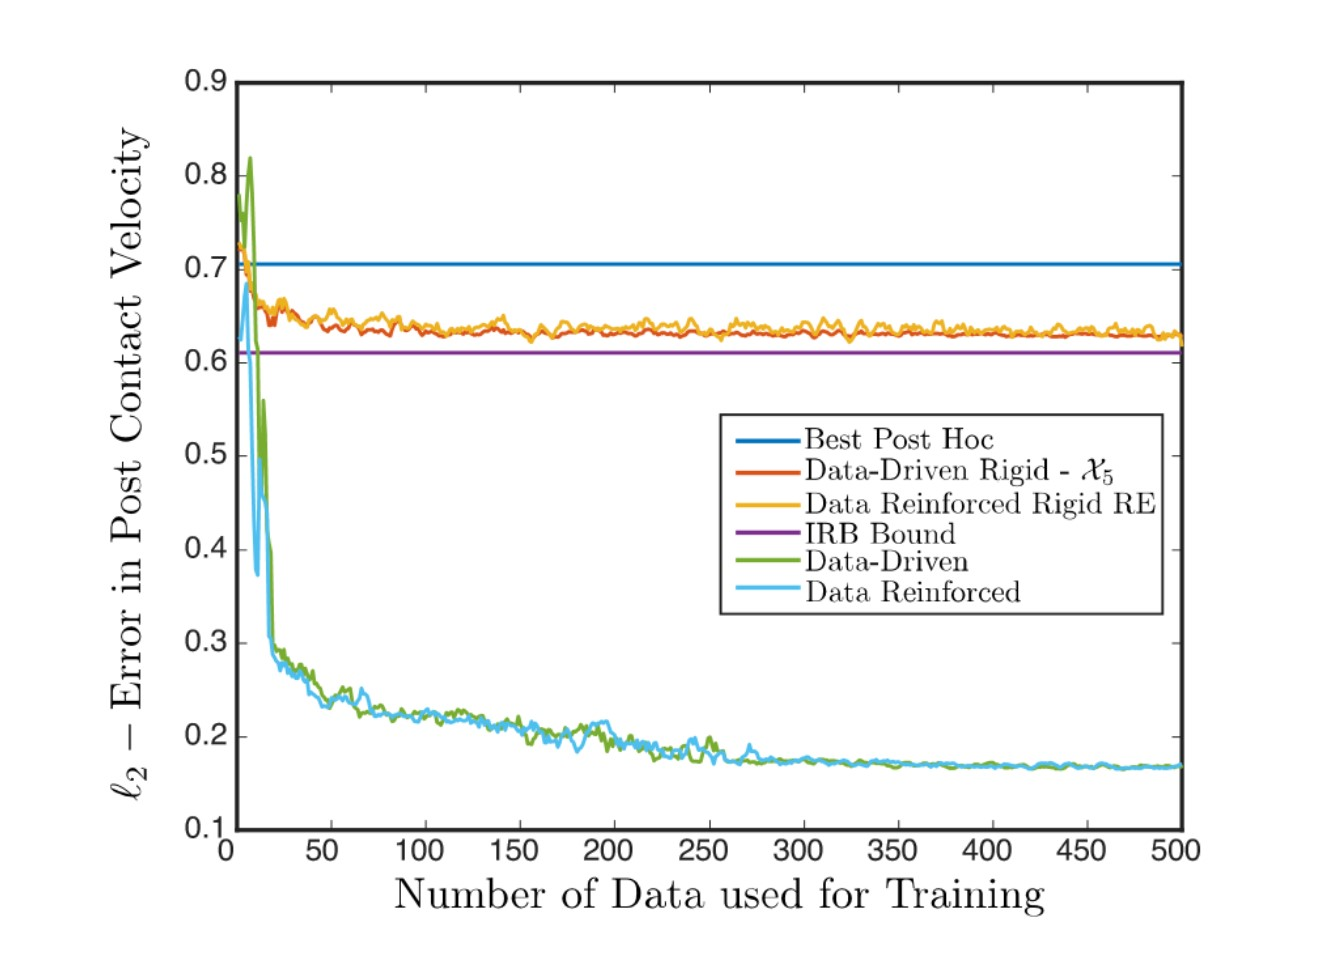
\includegraphics[scale=0.45]{nima1.jpg}
        \caption{Classic IRB\cite{nimaPaper}}
        \label{fig:cIRB}
    \end{subfigure}
    \quad
    \begin{subfigure}[b]{0.45\linewidth}
       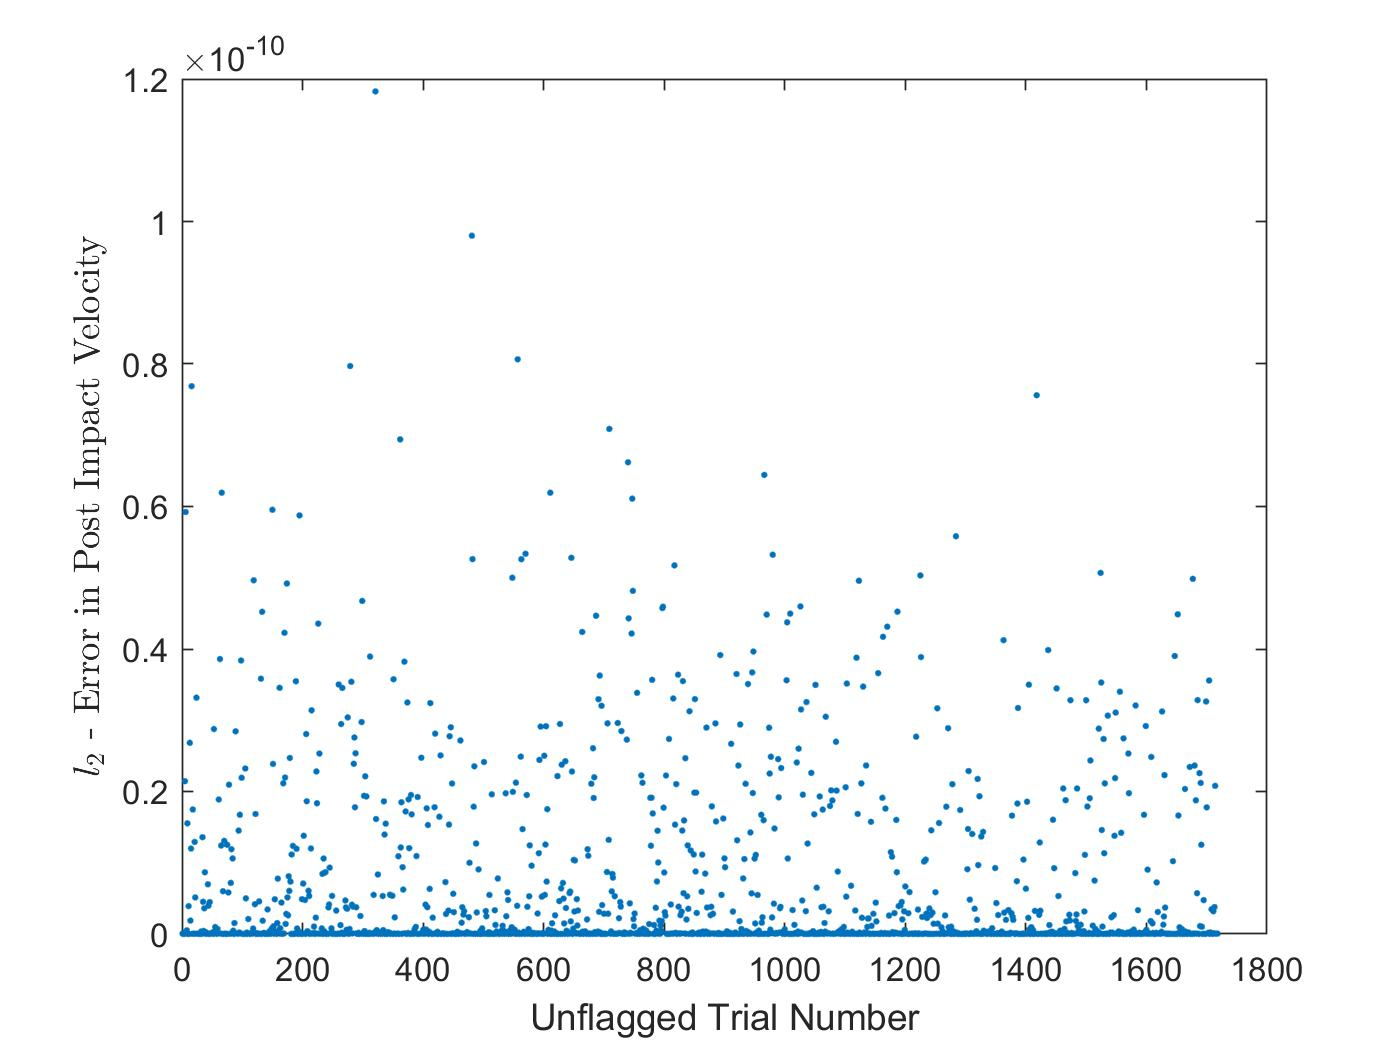
\includegraphics[scale=0.12]{errorWidth.jpg}
        \caption{IRB with Width}
        \label{fig:wIRB}
    \end{subfigure}
\end{figure}


\bibliographystyle{plainnat}
\bibliography{references}

\end{document}
